\begin{frame}
	\frametitle{Pong - Diagrama}
	
    \begin{center}
        Visión general del sistema
    \end{center}
	
    \begin{center}
		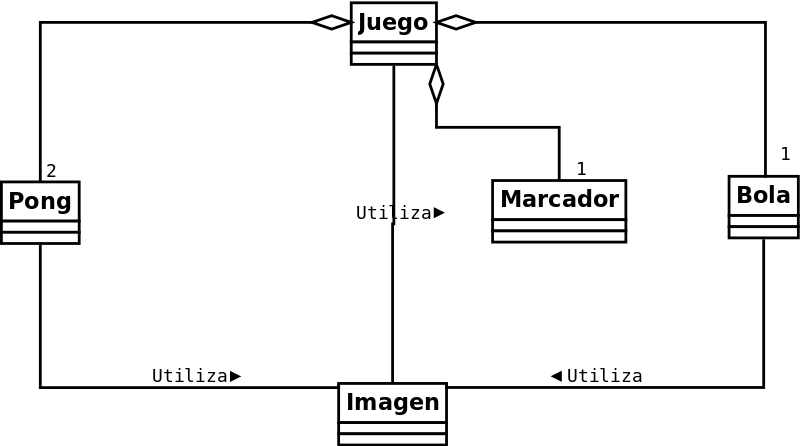
\includegraphics[scale=0.25]{img/modulos.png}
	\end{center}	

\end{frame}

\begin{frame}[fragile]
	\frametitle{Pong - Estructura del proyecto}
    
    \begin{columns}[c]
	\column{175pt}

\begin{verbatim}
|- pong
    |- makefile
    |- main.cpp
    |- motor
    |    |- fichero.c
    |    |- fichero.h
    |    |- (...)
    |
    |- multimedia
    |    |- imagen.png
    |    |- fuente.ttf
    |    |- (...)
\end{verbatim}
	
	\column{125pt}
	\begin{center}
		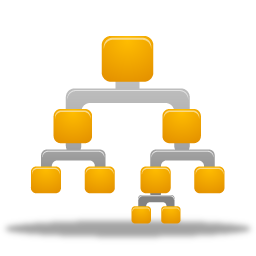
\includegraphics[scale=0.4]{img/Binary-tree-256.png}
	\end{center}	
	
    \end{columns}

\end{frame}

\begin{frame}
	\frametitle{Pong - Paso 1}
	
	\begin{block}{Objetivos}
		\begin{itemize}
			\item Inicializar SDL
			\item Crear una ventana
			\item Esperar evento de salida
			\item Cerrar SDL
		\end{itemize}            
	\end{block}

\end{frame}

\begin{frame}
	\frametitle{Pong - Paso 1}
	
    \begin{center}
        \textbf{¡Hora de currar!}
    \end{center}
	
    \begin{center}
		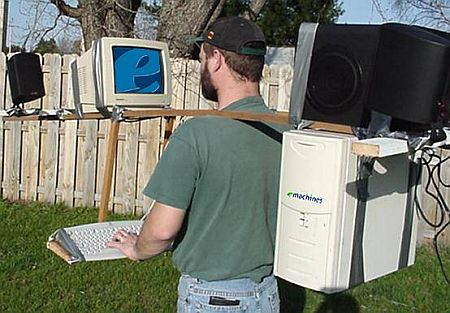
\includegraphics[scale=0.4]{img/currar-1.jpg}
    \end{center}	

\end{frame}

\begin{frame}
	\frametitle{Pong - Paso 1}
	
    \begin{center}
        \textbf{Resultado}
    \end{center}
	
    \begin{center}
		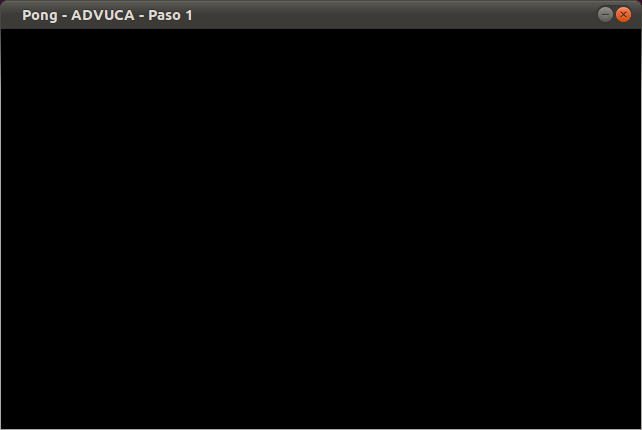
\includegraphics[scale=0.4]{img/pong-advuca-1.png}
    \end{center}	

\end{frame}

\begin{frame}
	\frametitle{Pong - Paso 2}
	
	\begin{block}{Objetivos}
		\begin{itemize}
			\item Módulo de carga y dibujado de imágenes
			\item Cargar mesa de juego
		\end{itemize}            
	\end{block}

\end{frame}

\begin{frame}
	\frametitle{Pong - Paso 2}
	
    \begin{center}
        \textbf{¡Hora de currar!}
    \end{center}
	
    \begin{center}
		
\includegraphics[scale=0.4]{img/currar-2.jpg}
	\end{center}	

\end{frame}

\begin{frame}
	\frametitle{Pong - Paso 2}
	
    \begin{center}
        \textbf{Resultado}
    \end{center}
	
    \begin{center}
		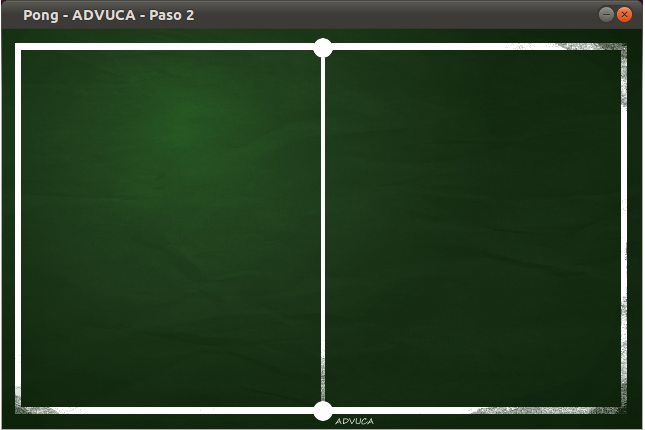
\includegraphics[scale=0.4]{img/pong-advuca-2.png}
	\end{center}	

\end{frame}

\begin{frame}
	\frametitle{Pong - Paso 3}
	
	\begin{block}{Objetivos}
		\begin{itemize}
			\item Módulo para las palas
			\item Control de la pala del jugador 1
			\item Control de FPS
		\end{itemize}            
	\end{block}

\end{frame}

\begin{frame}
	\frametitle{Pong - Paso 3}
	
    \begin{center}
        \textbf{¡Hora de currar!}
    \end{center}
	
    \begin{center}
		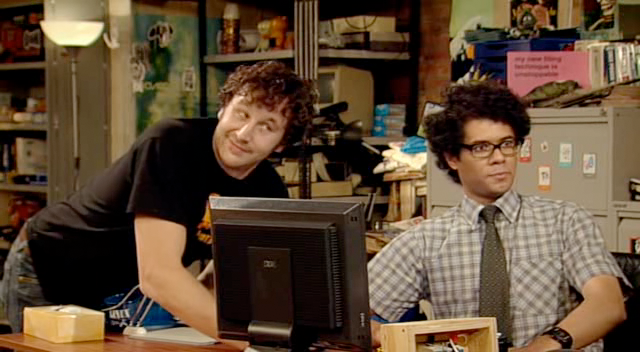
\includegraphics[scale=0.4]{img/currar-6.png}
	\end{center}	

\end{frame}

\begin{frame}
	\frametitle{Pong - Paso 3}
	
    \begin{center}
        \textbf{Resultado}
    \end{center}
	
    \begin{center}
		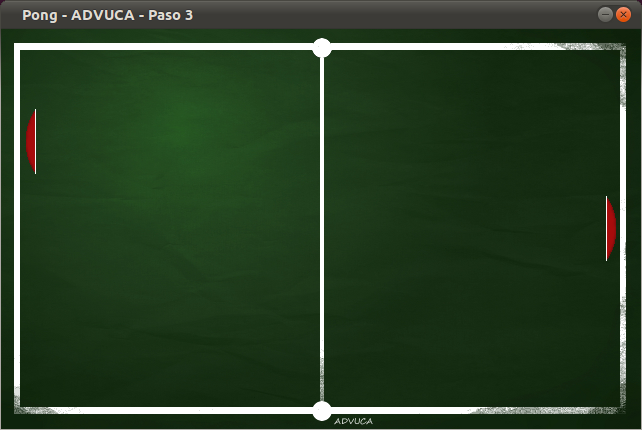
\includegraphics[scale=0.4]{img/pong-advuca-3.png}
	\end{center}	

\end{frame}

\begin{frame}
	\frametitle{Pong - Paso 4}
	
	\begin{block}{Objetivos}
		\begin{itemize}
			\item Módulo de la pelota
			\item Rebote básico de la pelota en bordes
			\item La pelota atraviesa las palas (por ahora)
		\end{itemize}            
	\end{block}

\end{frame}

\begin{frame}
	\frametitle{Pong - Paso 4}
	
    \begin{center}
        \textbf{¡Hora de currar!}
    \end{center}
	
    \begin{center}
		
\includegraphics[scale=0.4]{img/currar-4.jpg}
	\end{center}	

\end{frame}

\begin{frame}
	\frametitle{Pong - Paso 4}
	
    \begin{center}
        \textbf{Resultado}
    \end{center}
	
    \begin{center}
		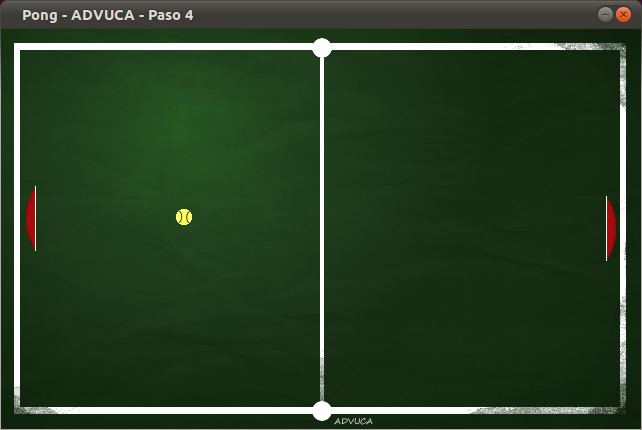
\includegraphics[scale=0.4]{img/pong-advuca-4.png}
	\end{center}	

\end{frame}

\begin{frame}
	\frametitle{Pong - Paso 5}
	
	\begin{block}{Objetivos}
		\begin{itemize}
			\item Colisión con las palas
			\item Inteligencia artificial
			\item La IA sigue a la pelota en el eje Y
		\end{itemize}            
	\end{block}

\end{frame}

\begin{frame}
	\frametitle{Pong - Paso 5}
	
    \begin{center}
        \textbf{¡Hora de currar!}
    \end{center}
	
    \begin{center}
		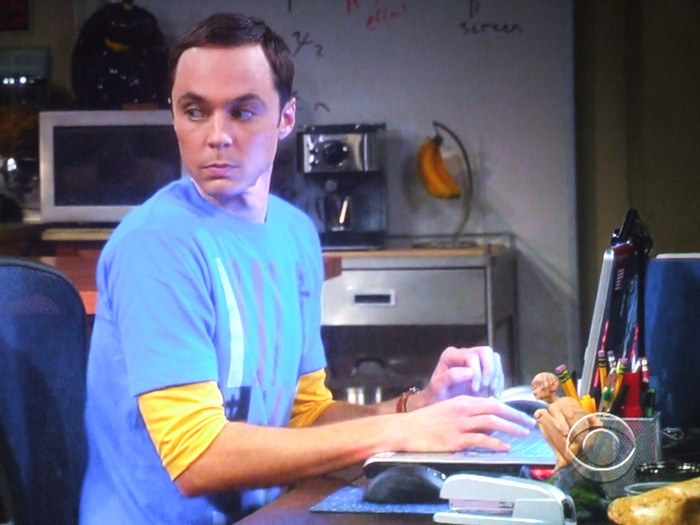
\includegraphics[scale=0.3]{img/currar-5.jpg}
	\end{center}	

\end{frame}

\begin{frame}
	\frametitle{Pong - Paso 5}
	
    \begin{center}
        \textbf{Resultado}
    \end{center}
	
    \begin{center}
		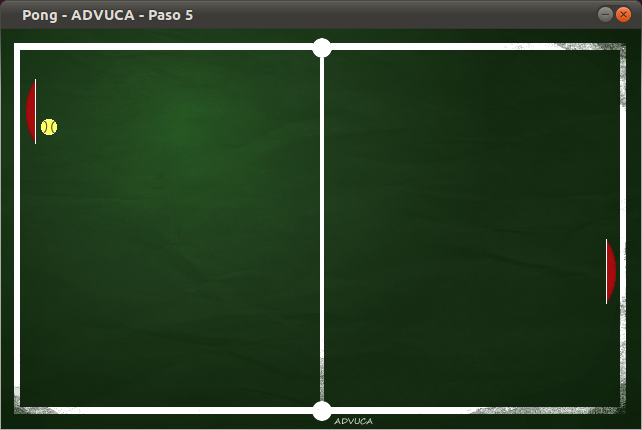
\includegraphics[scale=0.4]{img/pong-advuca-5.png}
	\end{center}	

\end{frame}

\begin{frame}
	\frametitle{Pong - Paso 6}
	
	\begin{block}{Objetivos}
		\begin{itemize}
			\item Creación del módulo marcador
			\item Si el jugador golpea la bola, suma un punto
			\item Se mantiene el récord de golpeos
			\item El marcador se reinicia si el jugador falla
		\end{itemize}            
	\end{block}

\end{frame}

\begin{frame}
	\frametitle{Pong - Paso 6}
	
    \begin{center}
        \textbf{¡Hora de currar!}
    \end{center}
	
    \begin{center}
		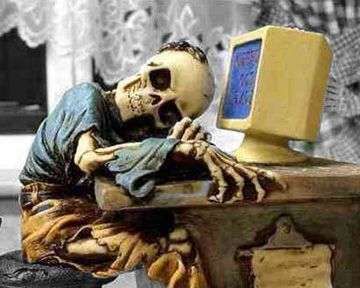
\includegraphics[scale=0.7]{img/currar-3.jpg}
	\end{center}	

\end{frame}

\begin{frame}
	\frametitle{Pong - Paso 6}
	
    \begin{center}
        \textbf{Resultado}
    \end{center}
	
    \begin{center}
		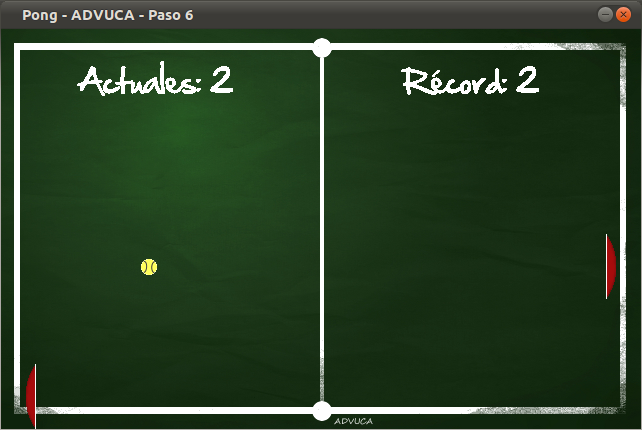
\includegraphics[scale=0.4]{img/pong-advuca-6.png}
	\end{center}	

\end{frame}
